% generated by scripts/trace_montecarlo.py -- do not edit by hand
\begin{figure}[!htbp]
\centering
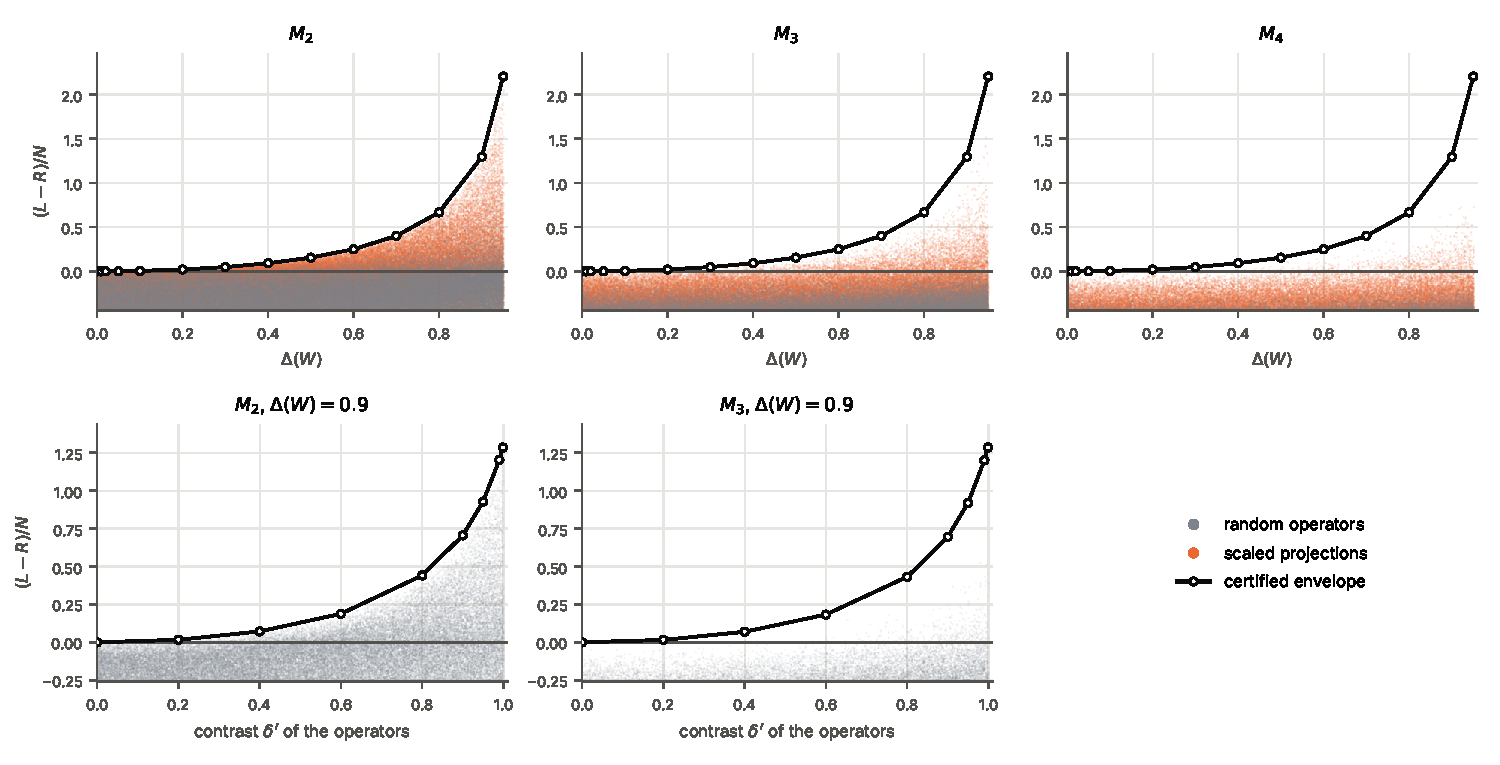
\includegraphics[width=\textwidth]{mc_01_gardner.pdf}
\caption[]{Item 1, $|\varphi(X)|\le\varphi(|X|)$: random samples and the computed envelope (a certified lower bound); top: against $\Delta(W)$, bottom: against the contrast $\delta^\prime$ of the operators at $\Delta(W)=0.9$.}
\label{fig:mc-gardner}
\end{figure}

\begin{figure}[!htbp]
\centering
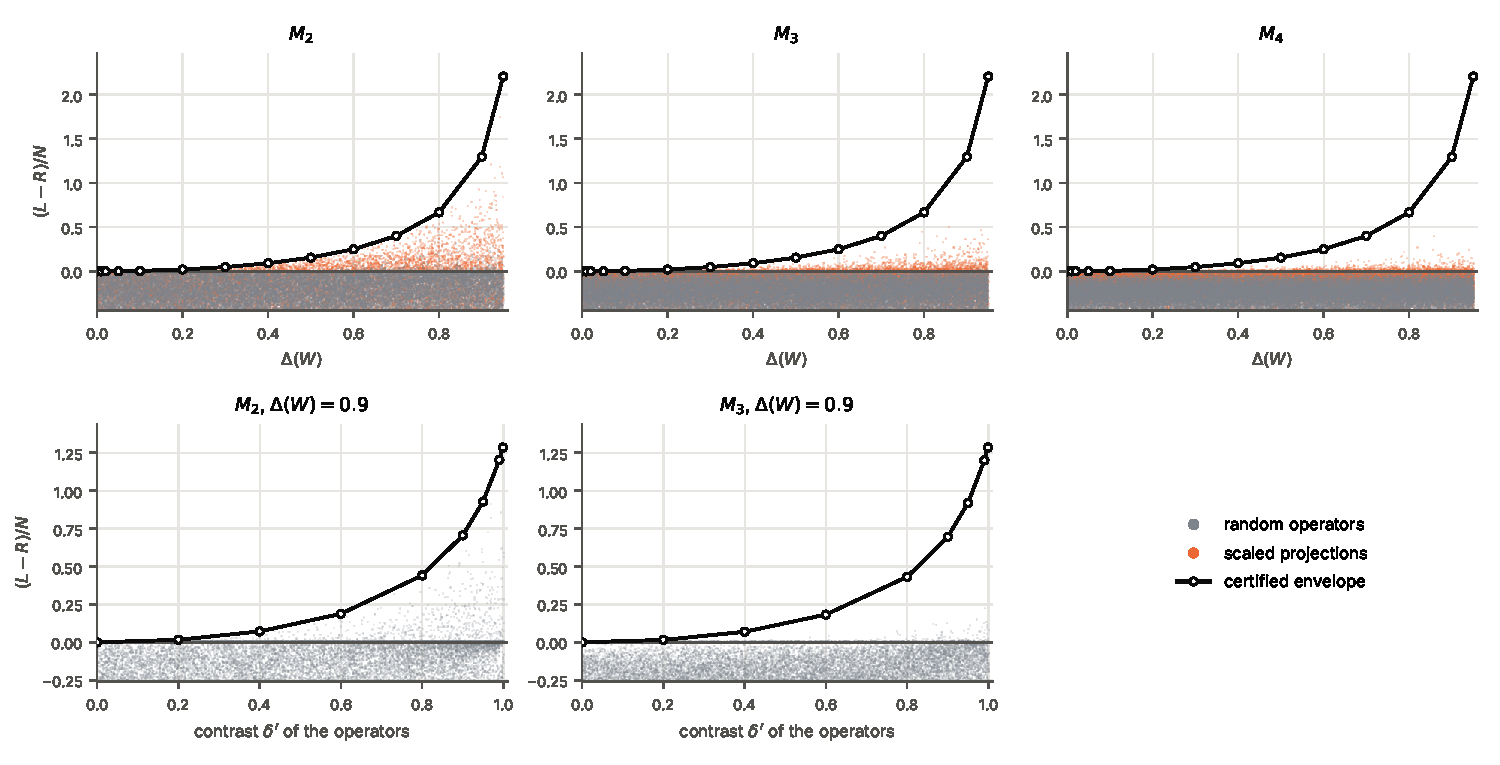
\includegraphics[width=\textwidth]{mc_02_triangle.pdf}
\caption[]{Item 2, $\varphi(|X+Y|)\le\varphi(|X|)+\varphi(|Y|)$: random samples and the computed envelope (a certified lower bound); top: against $\Delta(W)$, bottom: against the contrast $\delta^\prime$ of the operators at $\Delta(W)=0.9$.}
\label{fig:mc-triangle}
\end{figure}

\begin{figure}[!htbp]
\centering
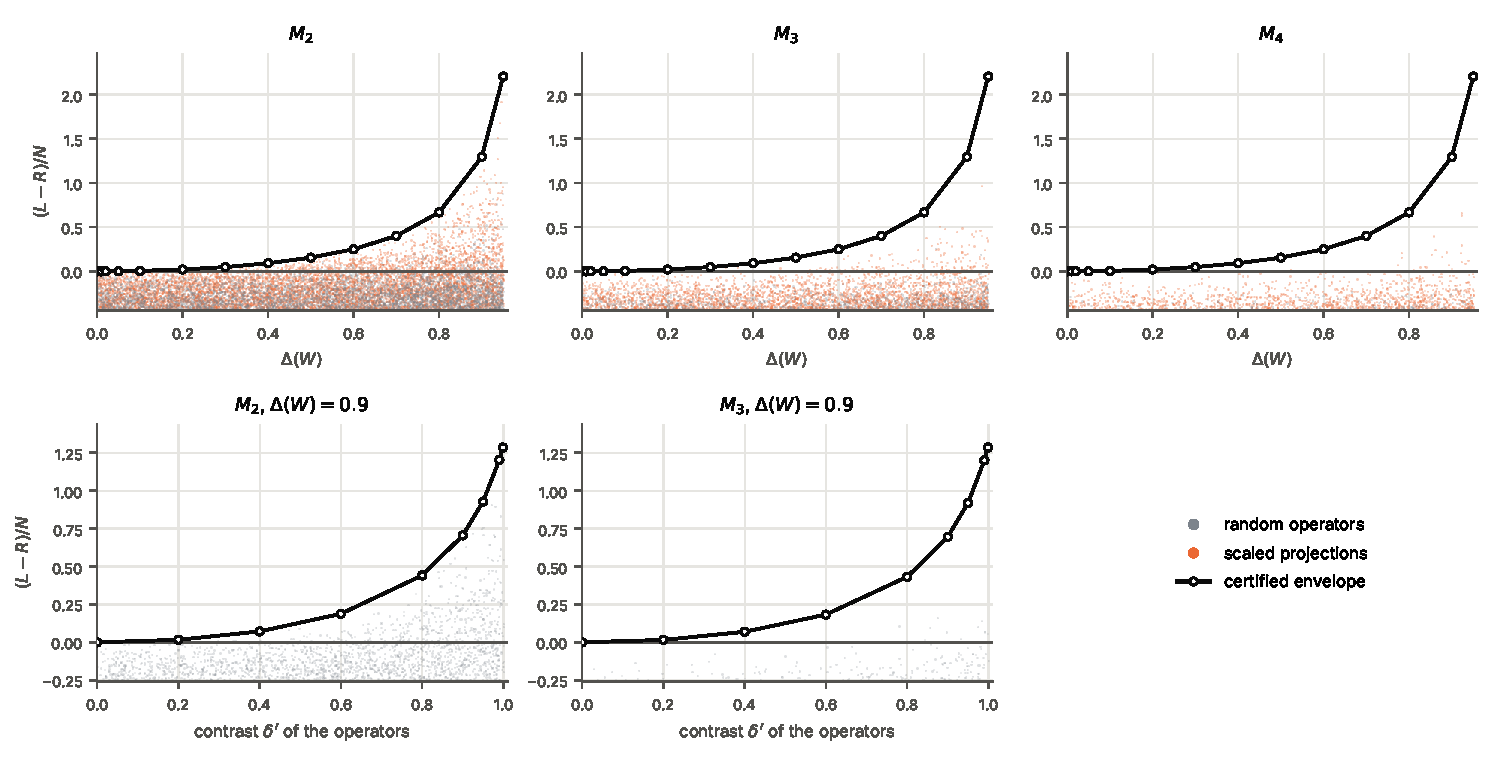
\includegraphics[width=\textwidth]{mc_03_realpart.pdf}
\caption[]{Item 3, $\varphi(A+A^*)\le2\varphi(|A^*|)$: random samples and the computed envelope (a certified lower bound); top: against $\Delta(W)$, bottom: against the contrast $\delta^\prime$ of the operators at $\Delta(W)=0.9$.}
\label{fig:mc-realpart}
\end{figure}

\begin{figure}[!htbp]
\centering
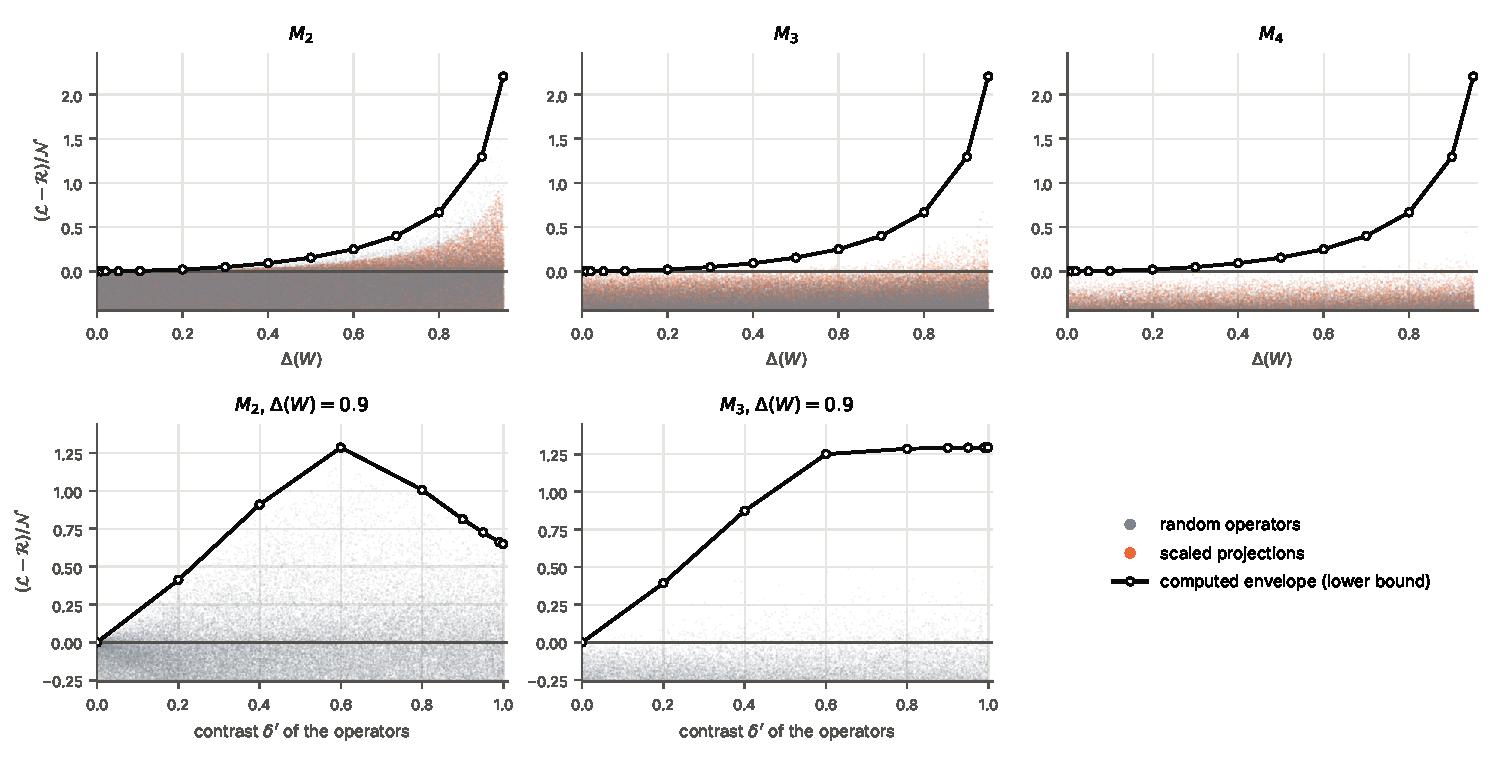
\includegraphics[width=\textwidth]{mc_04_square.pdf}
\caption[]{Item 4, $|\varphi(A^2)|\le\varphi(A^*A)$: random samples and the computed envelope (a certified lower bound); top: against $\Delta(W)$, bottom: against the contrast $\delta^\prime$ of the operators at $\Delta(W)=0.9$.}
\label{fig:mc-square}
\end{figure}

\begin{figure}[!htbp]
\centering
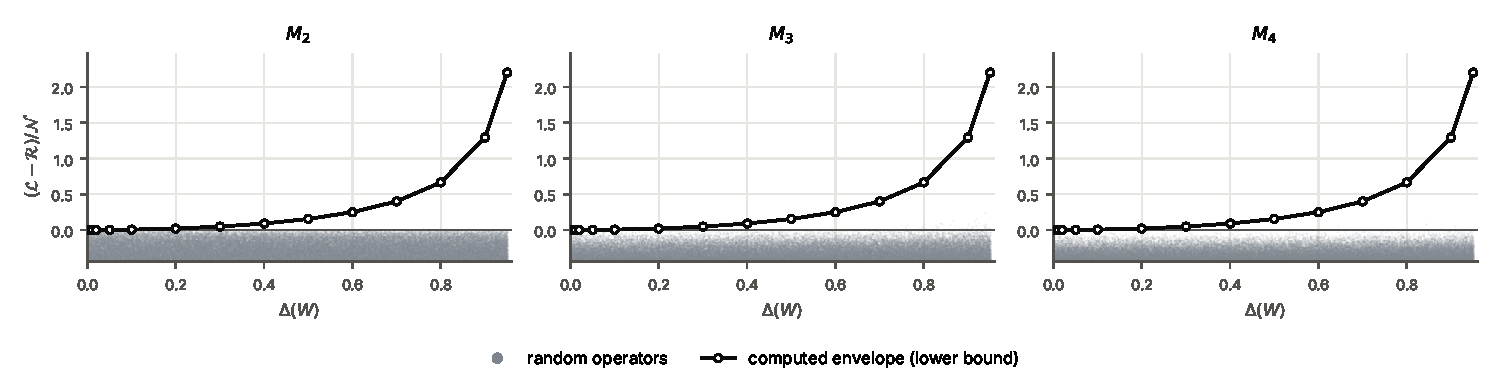
\includegraphics[width=\textwidth]{mc_05_metric.pdf}
\caption[]{Item 5, $\varphi(|P-R|)\le\varphi(|P-Q|)+\varphi(|Q-R|)$: random samples and the computed envelope (a certified lower bound) against $\Delta(W)$.}
\label{fig:mc-metric}
\end{figure}

\begin{figure}[!htbp]
\centering
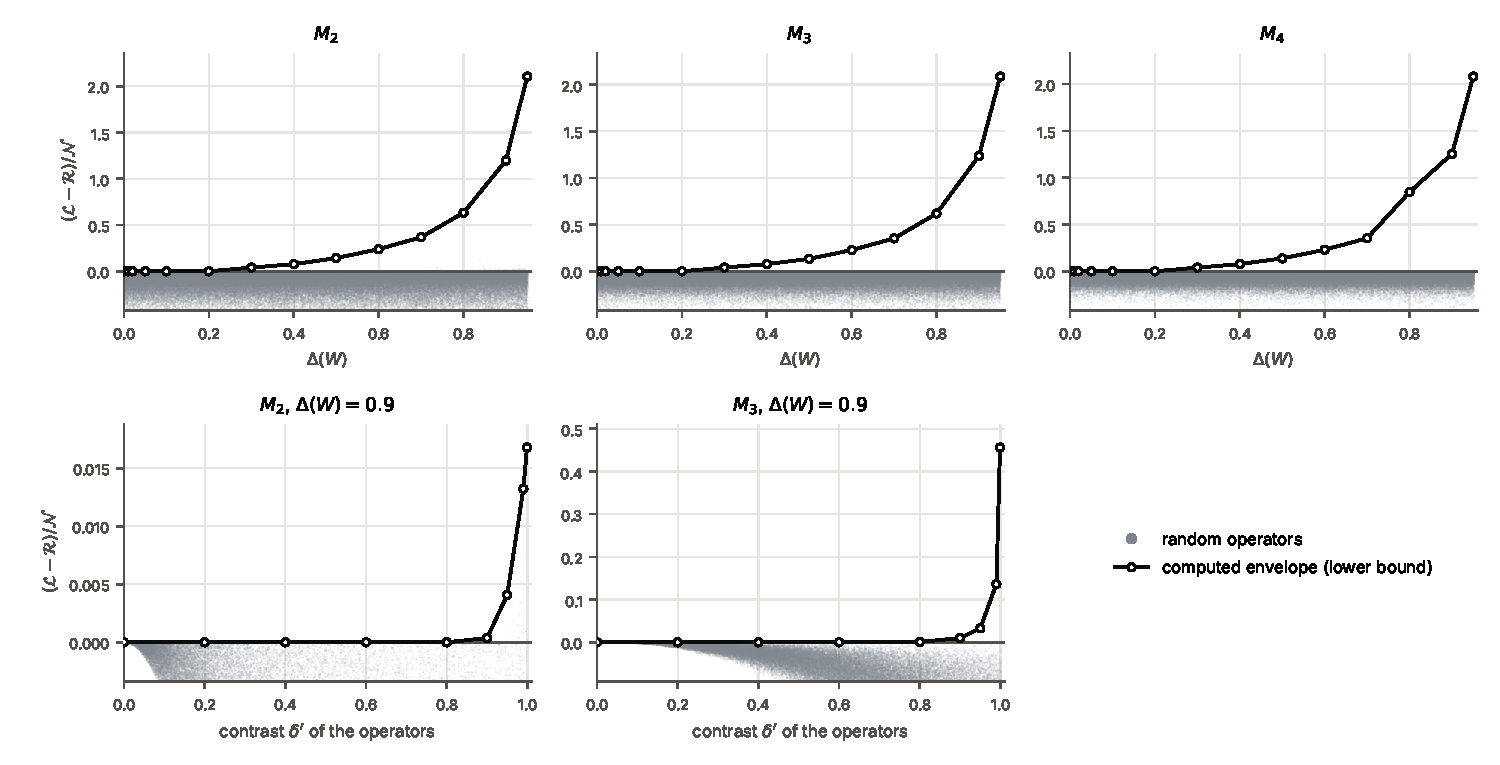
\includegraphics[width=\textwidth]{mc_06_sgm.pdf}
\caption[]{Item 6, $\varphi(A\natural B)\le\sqrt{\varphi(A)\varphi(B)}$: random samples and the computed envelope (a certified lower bound); top: against $\Delta(W)$, bottom: against the contrast $\delta^\prime$ of the operators at $\Delta(W)=0.9$.}
\label{fig:mc-sgm}
\end{figure}

\begin{figure}[!htbp]
\centering
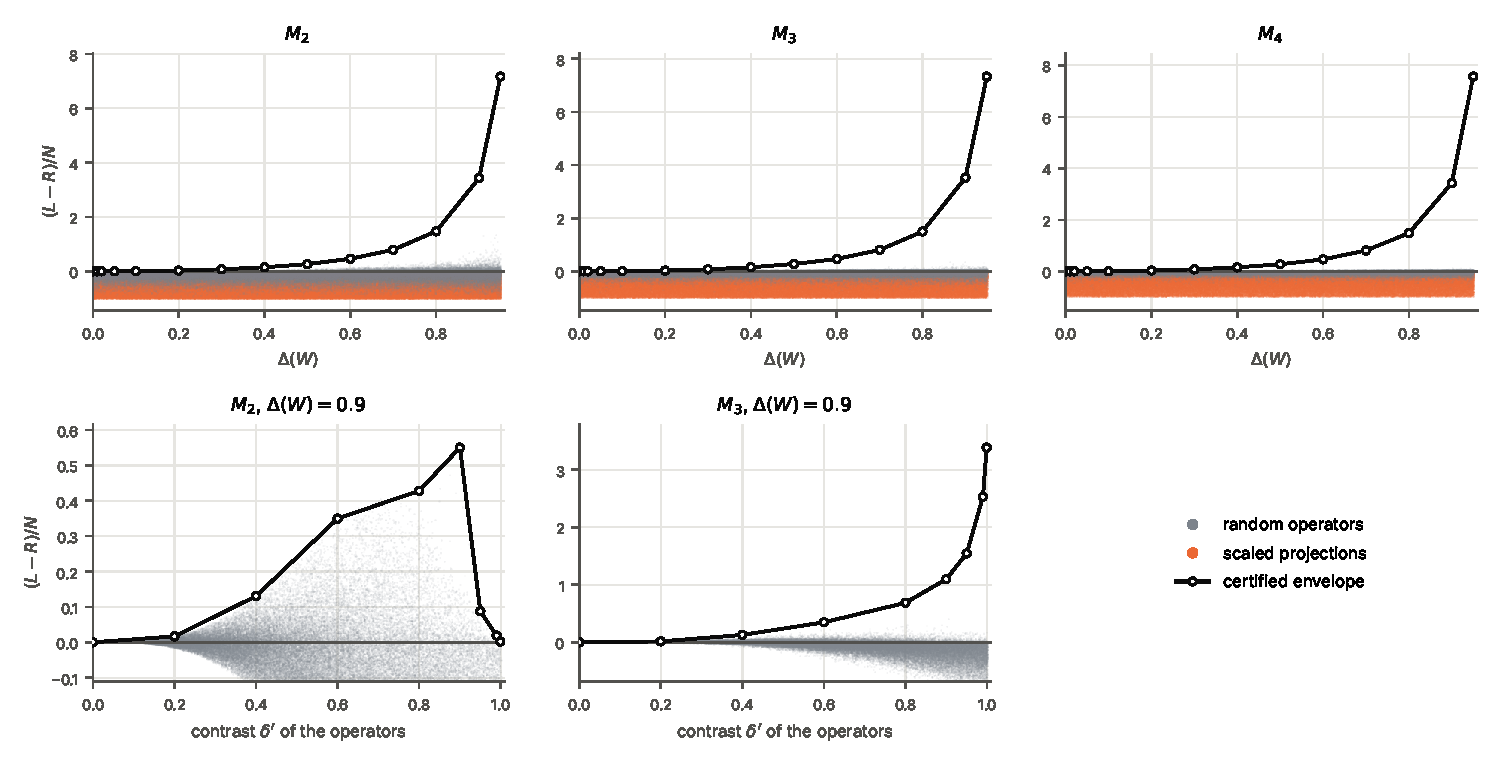
\includegraphics[width=\textwidth]{mc_07_alt.pdf}
\caption[]{Item 7, $\varphi((B^{1/2}AB^{1/2})^2)\le\varphi(BA^2B)$: random samples and the computed envelope (a certified lower bound); top: against $\Delta(W)$, bottom: against the contrast $\delta^\prime$ of the operators at $\Delta(W)=0.9$.}
\label{fig:mc-alt}
\end{figure}

\begin{figure}[!htbp]
\centering
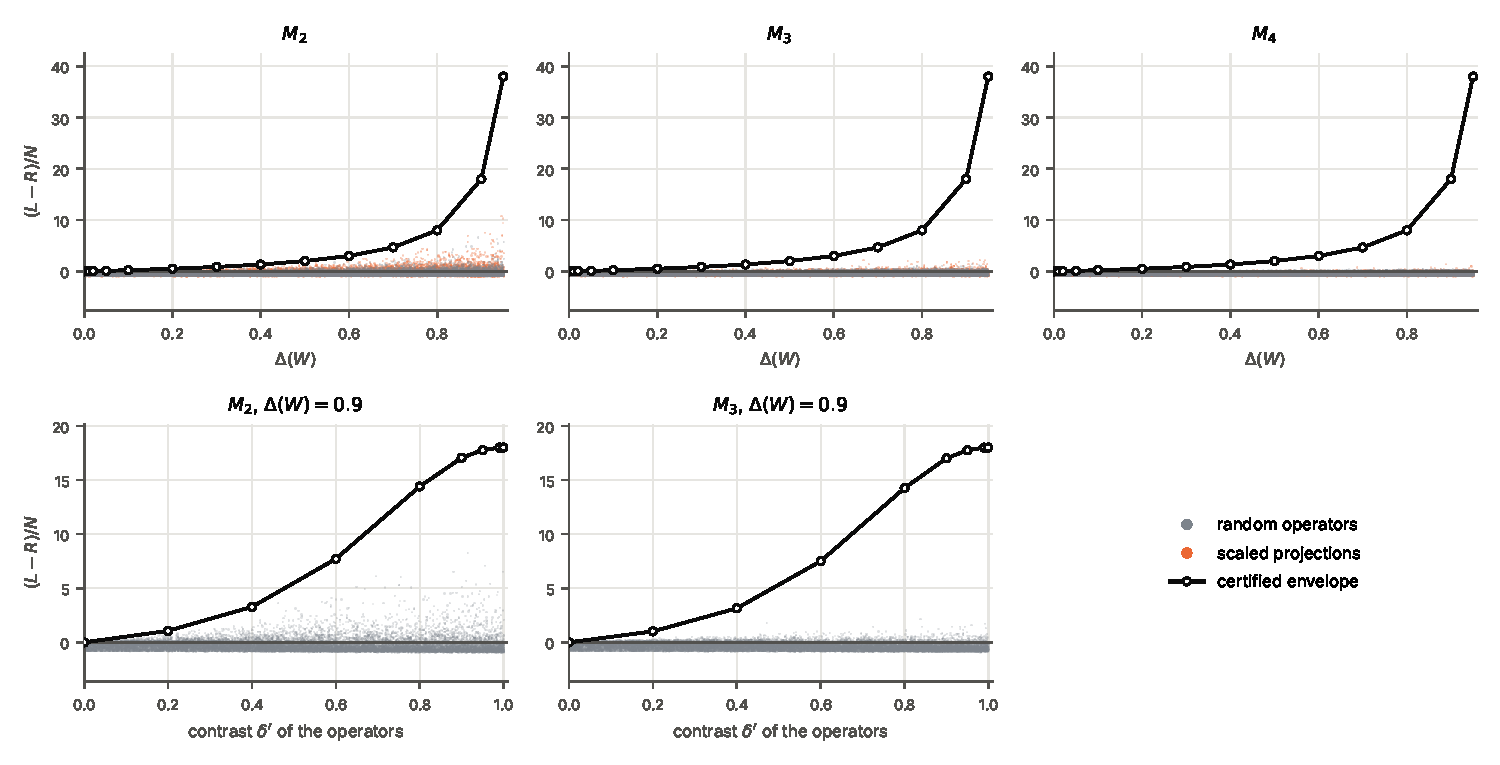
\includegraphics[width=\textwidth]{mc_08_young.pdf}
\caption[]{Item 8, $\varphi(|AB^*|)\le\frac12\varphi(|A|^2)+\frac12\varphi(|B|^2)$: random samples and the computed envelope (a certified lower bound); top: against $\Delta(W)$, bottom: against the contrast $\delta^\prime$ of the operators at $\Delta(W)=0.9$.}
\label{fig:mc-young}
\end{figure}

\begin{figure}[!htbp]
\centering
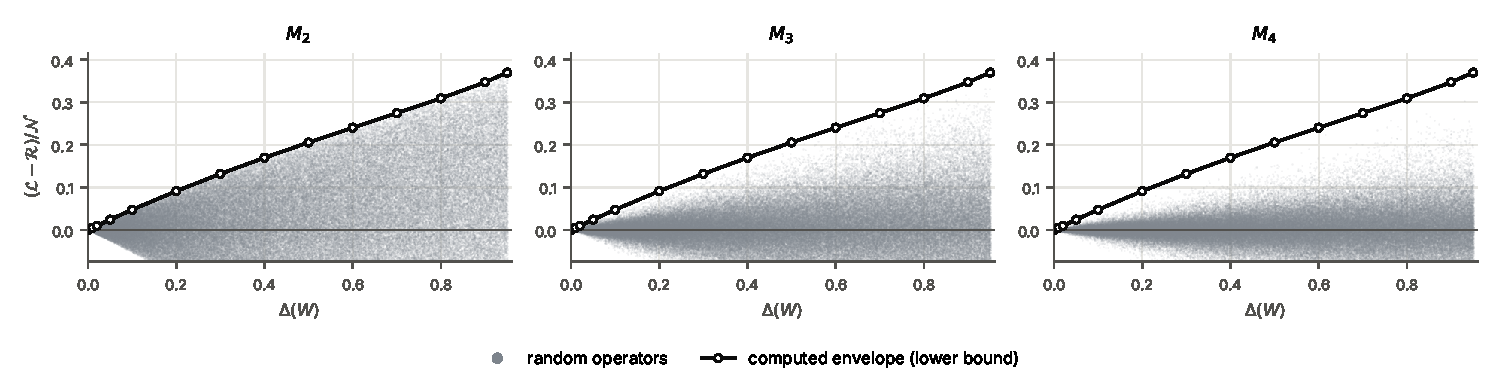
\includegraphics[width=\textwidth]{mc_09_projections.pdf}
\caption[]{Item 9, $\varphi(PQ+QP)\le2\varphi(QPQ)$: random samples and the computed envelope (a certified lower bound) against $\Delta(W)$.}
\label{fig:mc-projections}
\end{figure}

\begin{figure}[!htbp]
\centering
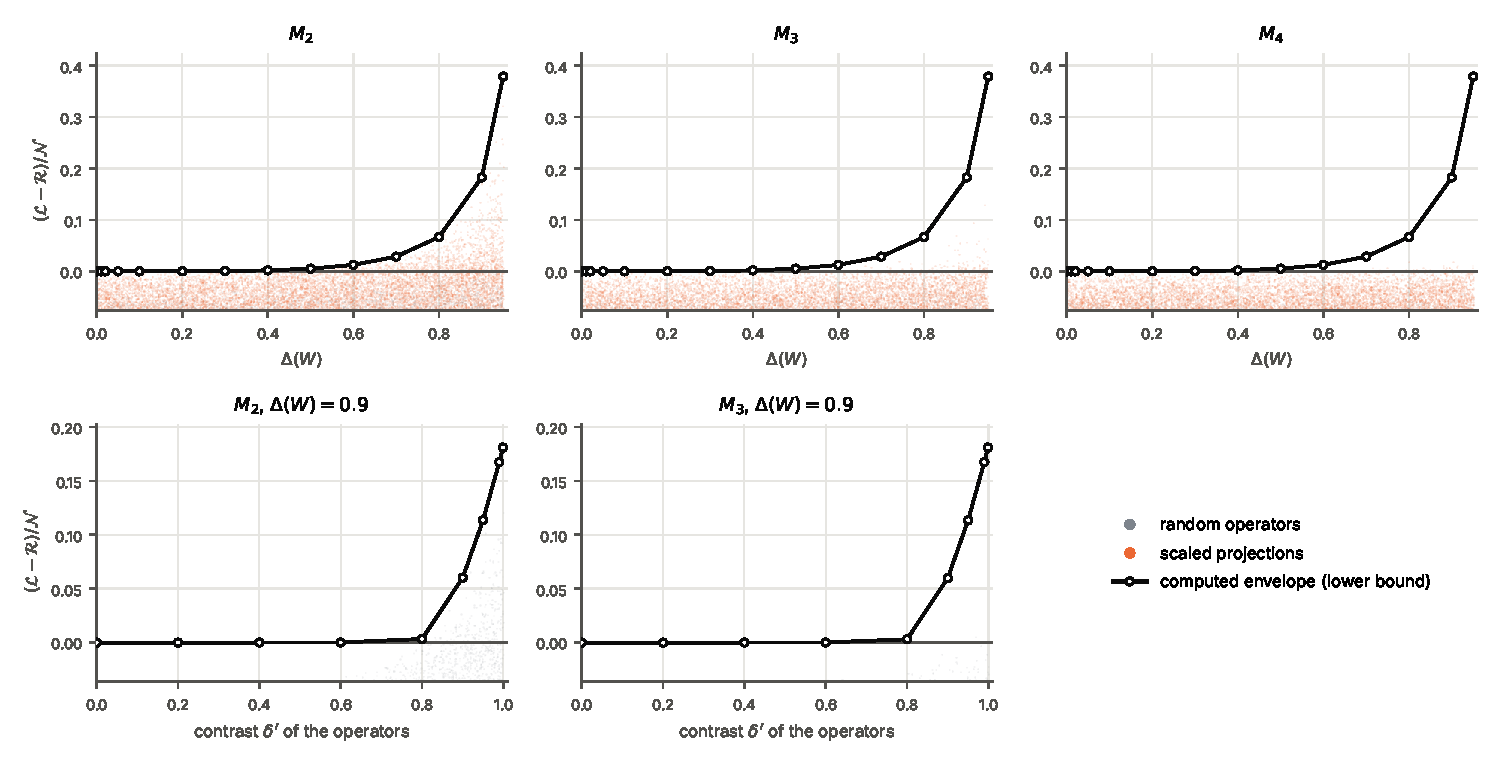
\includegraphics[width=\textwidth]{mc_10_monotone.pdf}
\caption[]{Item 10, $0\le A\le B\Rightarrow\varphi(A^2)\le\varphi(B^2)$: random samples and the computed envelope (a certified lower bound); top: against $\Delta(W)$, bottom: against the contrast $\delta^\prime$ of the operators at $\Delta(W)=0.9$.}
\label{fig:mc-monotone}
\end{figure}

\begin{figure}[!htbp]
\centering
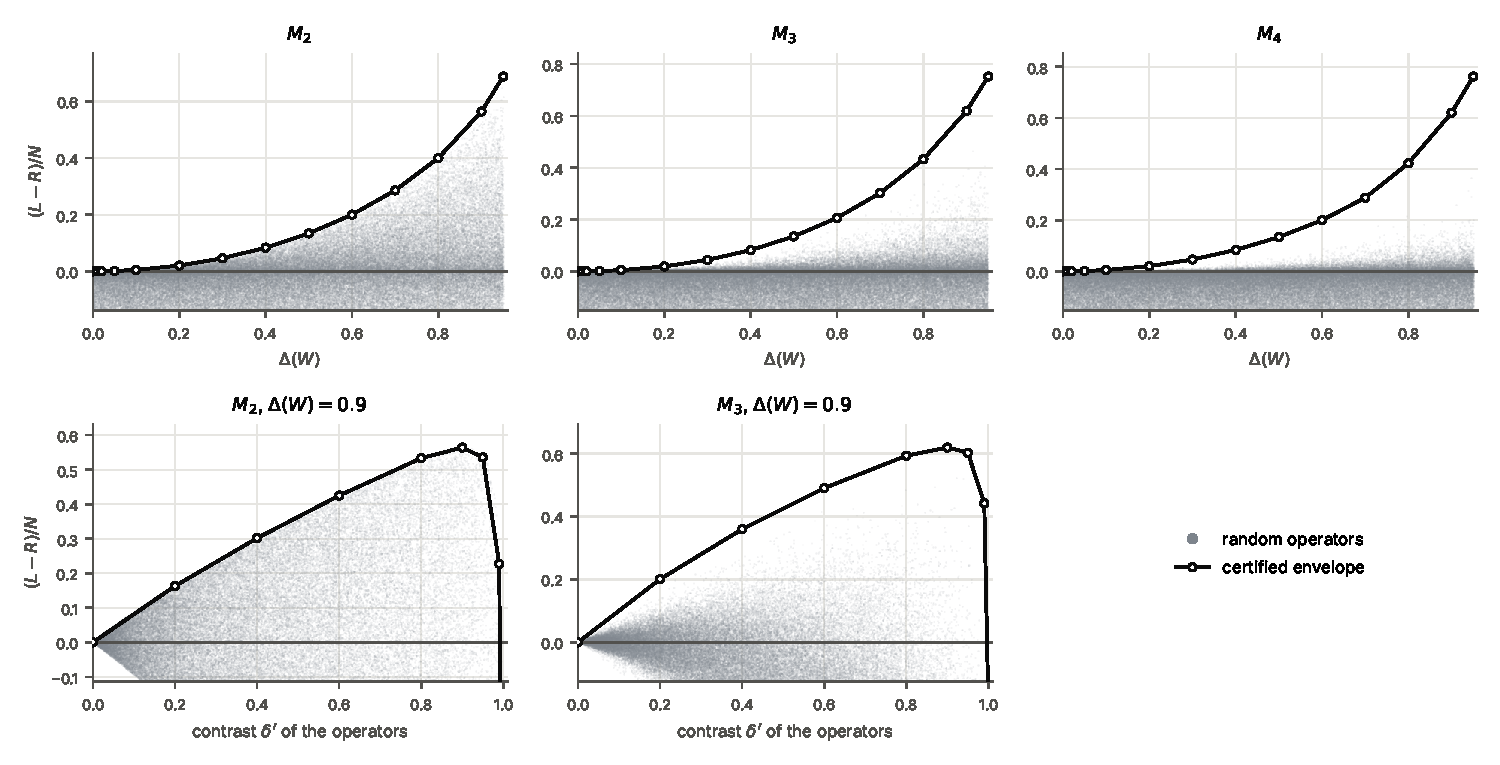
\includegraphics[width=\textwidth]{mc_11_det.pdf}
\caption[]{Item 11, $(\det A)^{1/n}\le\frac1n\varphi(A)$, $\varphi(1)=n$: random samples and the computed envelope (a certified lower bound); top: against $\Delta(W)$, bottom: against the contrast $\delta^\prime$ of the operators at $\Delta(W)=0.9$.}
\label{fig:mc-det}
\end{figure}

\begin{figure}[!htbp]
\centering
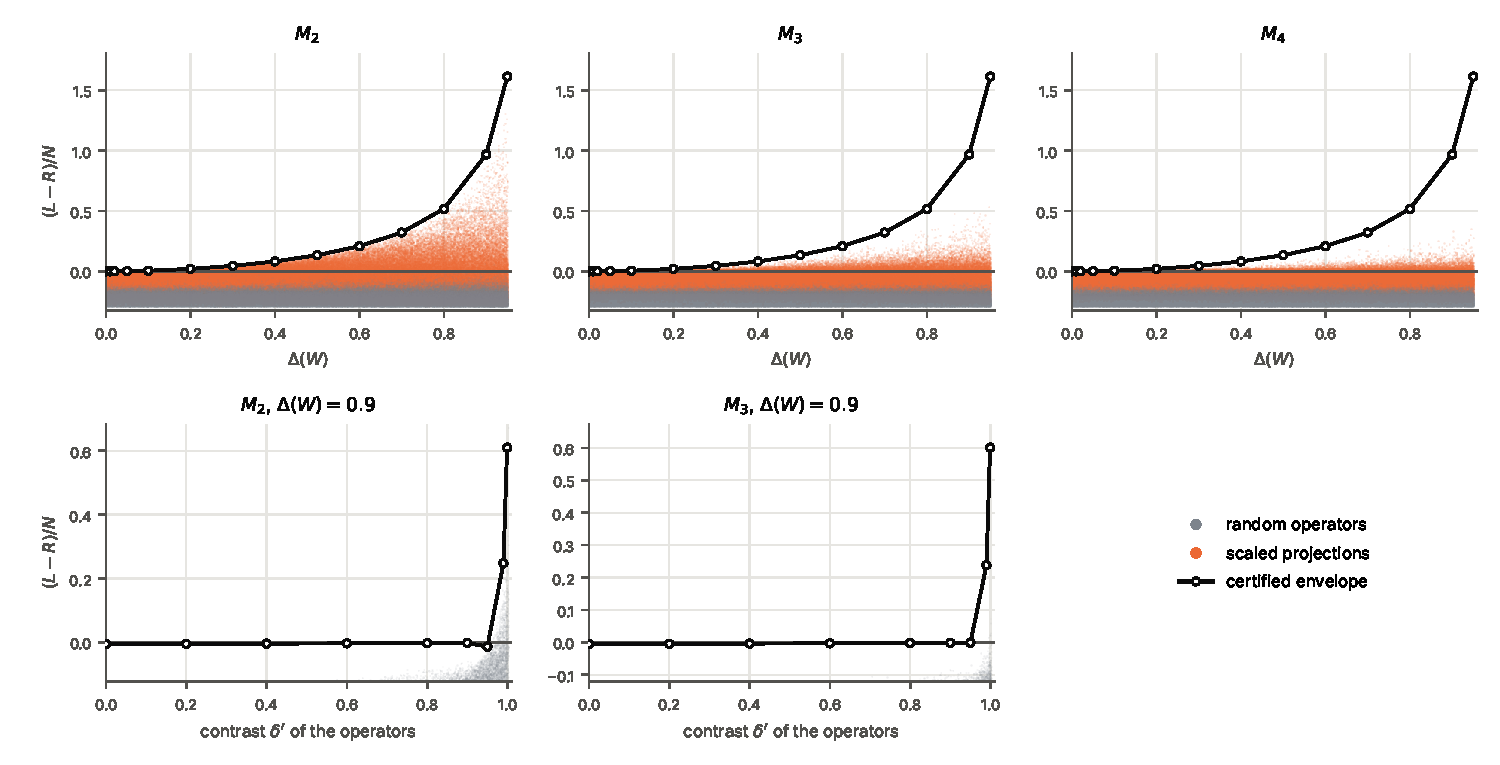
\includegraphics[width=\textwidth]{mc_12_subadd.pdf}
\caption[]{Item 12, $\varphi((A+B)^{1/2})\le\varphi(A^{1/2})+\varphi(B^{1/2})$: random samples and the computed envelope (a certified lower bound); top: against $\Delta(W)$, bottom: against the contrast $\delta^\prime$ of the operators at $\Delta(W)=0.9$.}
\label{fig:mc-subadd}
\end{figure}

\begin{figure}[!htbp]
\centering
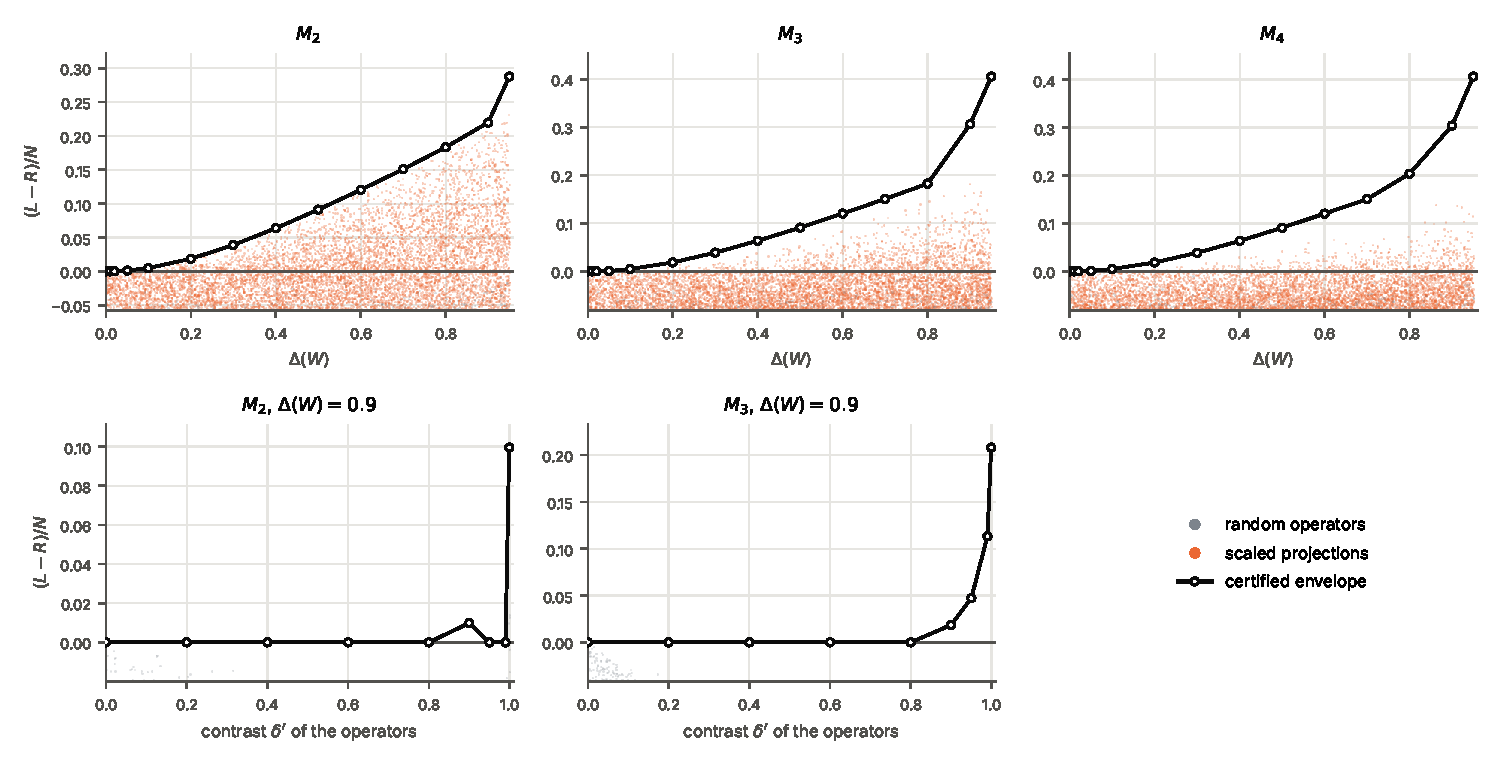
\includegraphics[width=\textwidth]{mc_13_powers.pdf}
\caption[]{Item 13, $\varphi(A+B-|A-B|)\le2\varphi(A^{1/4}B^{1/2}A^{1/4})$: random samples and the computed envelope (a certified lower bound); top: against $\Delta(W)$, bottom: against the contrast $\delta^\prime$ of the operators at $\Delta(W)=0.9$.}
\label{fig:mc-powers}
\end{figure}

\begin{figure}[!htbp]
\centering
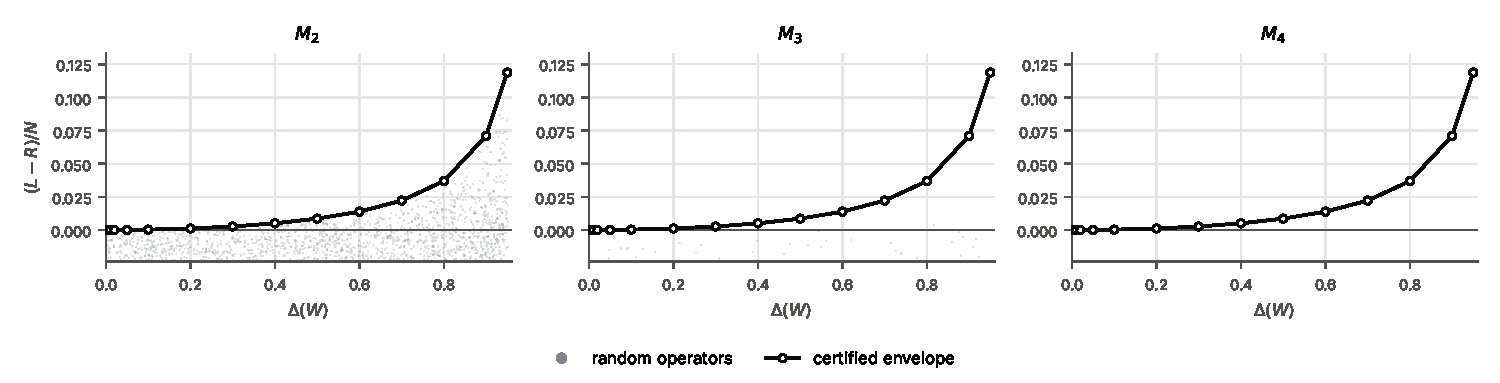
\includegraphics[width=\textwidth]{mc_14_holder.pdf}
\caption[]{Item 14, $|\varphi(PQ)|\le\varphi(P)^{1/3}\varphi(Q)^{2/3}$: random samples and the computed envelope (a certified lower bound) against $\Delta(W)$.}
\label{fig:mc-holder}
\end{figure}

\begin{figure}[!htbp]
\centering
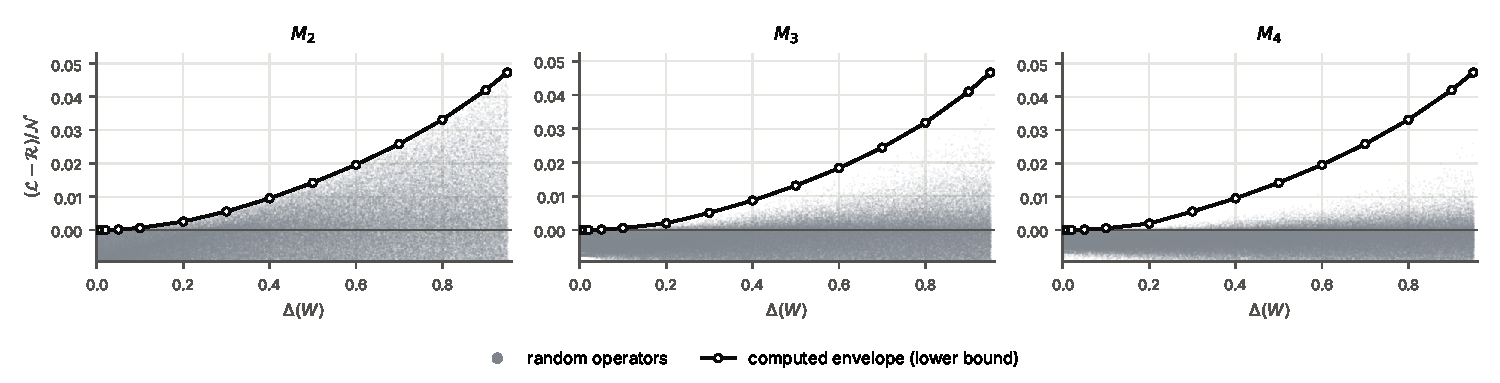
\includegraphics[width=\textwidth]{mc_15_gt.pdf}
\caption[]{Item 15, $\varphi(e^{P+Q})\le\varphi(e^{P/2}e^Qe^{P/2})$: random samples and the computed envelope (a certified lower bound) against $\Delta(W)$.}
\label{fig:mc-gt}
\end{figure}

\begin{figure}[!htbp]
\centering
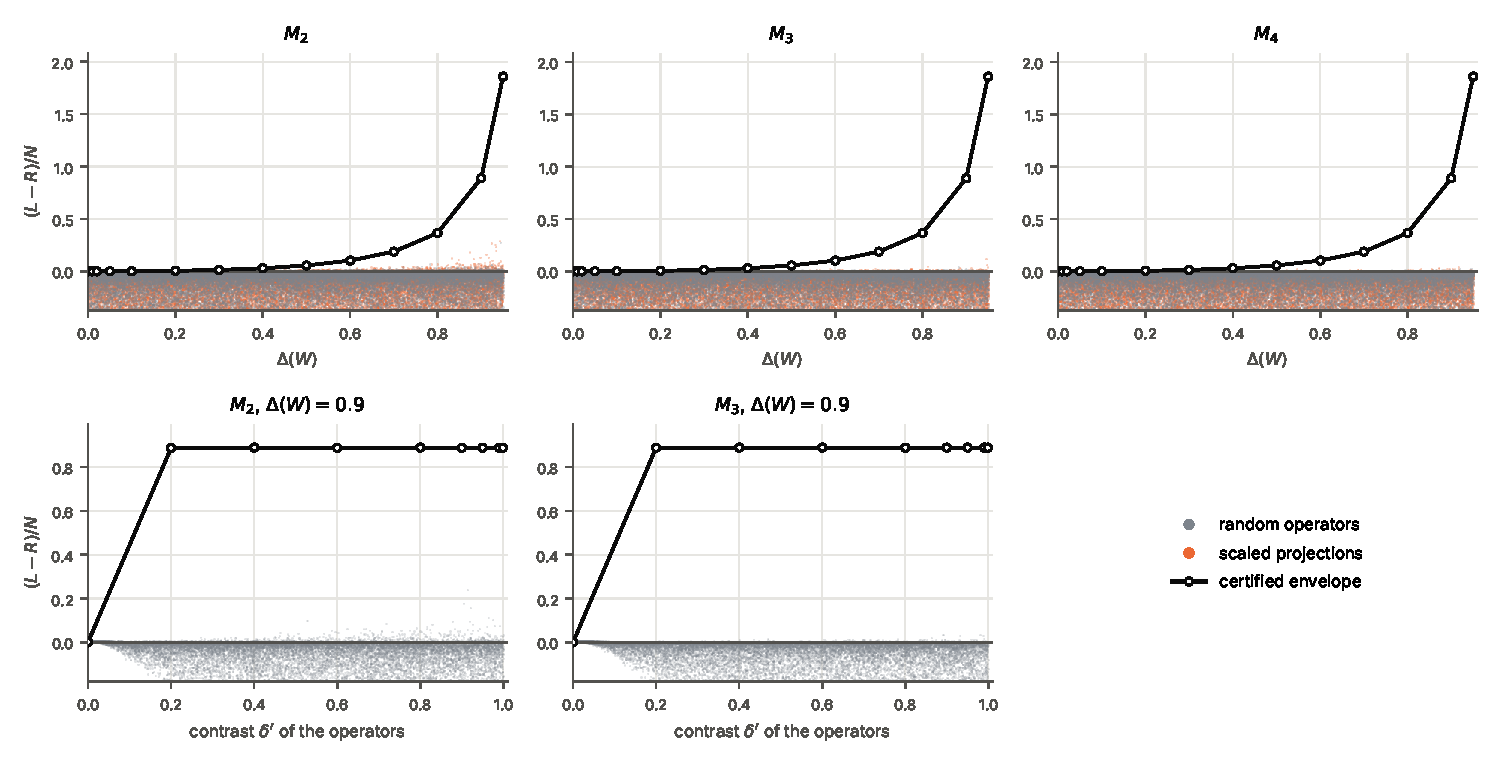
\includegraphics[width=\textwidth]{mc_16_pb.pdf}
\caption[]{Item 16, $\varphi(e^A)e^{\varphi(e^{A/2}Be^{A/2})/\varphi(e^A)}\le\varphi(e^{A+B})$: random samples and the computed envelope (a certified lower bound); top: against $\Delta(W)$, bottom: against the contrast $\delta^\prime$ of the operators at $\Delta(W)=0.9$.}
\label{fig:mc-pb}
\end{figure}

\begin{figure}[!htbp]
\centering
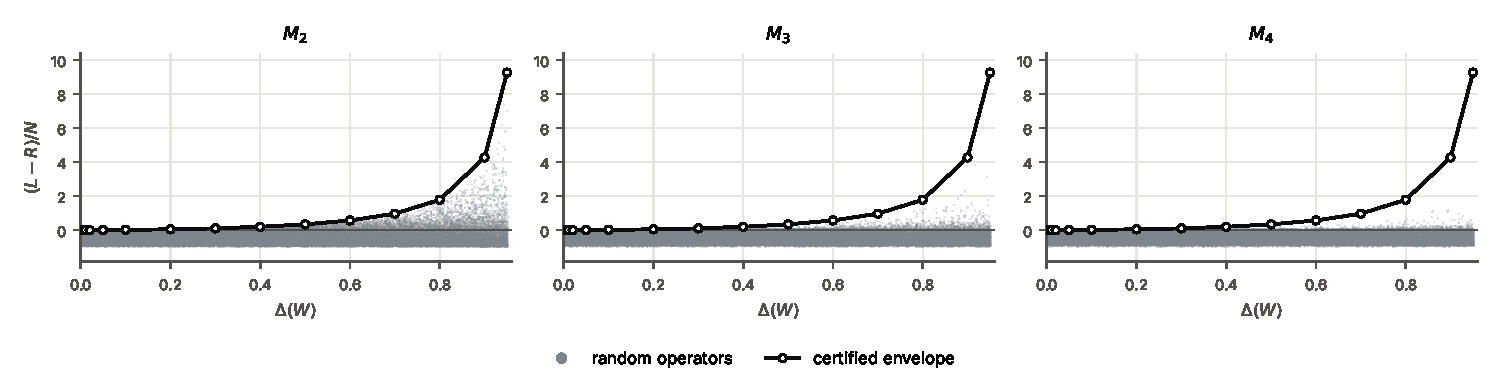
\includegraphics[width=\textwidth]{mc_17_pqp.pdf}
\caption[]{Item 17, $\varphi(PQP)\le\varphi(Q)$: random samples and the computed envelope (a certified lower bound) against $\Delta(W)$.}
\label{fig:mc-pqp}
\end{figure}

\begin{figure}[!htbp]
\centering
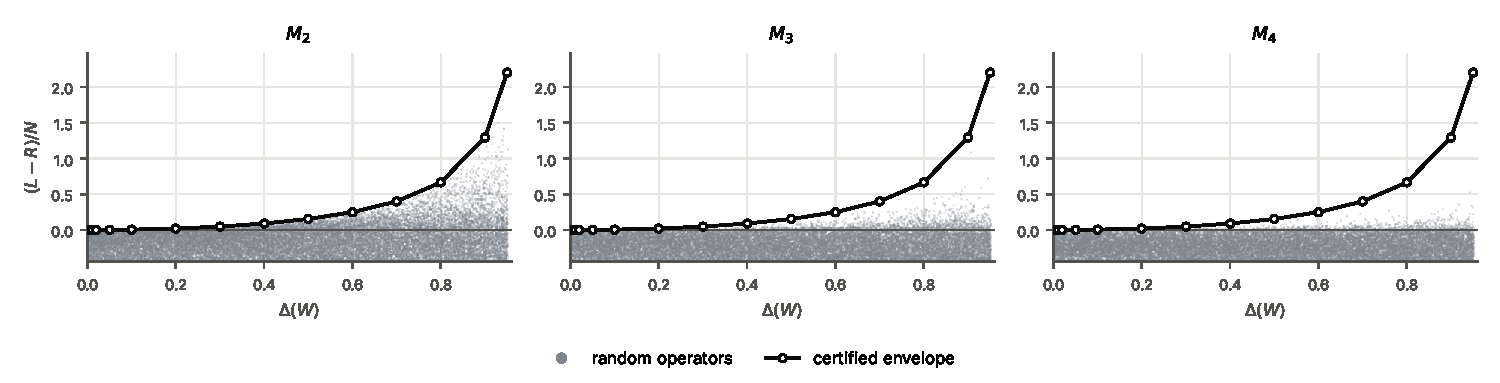
\includegraphics[width=\textwidth]{mc_18_absdiff.pdf}
\caption[]{Item 18, $\varphi(|P-Q|)\le\varphi(P+Q)$: random samples and the computed envelope (a certified lower bound) against $\Delta(W)$.}
\label{fig:mc-absdiff}
\end{figure}

\begin{figure}[!htbp]
\centering
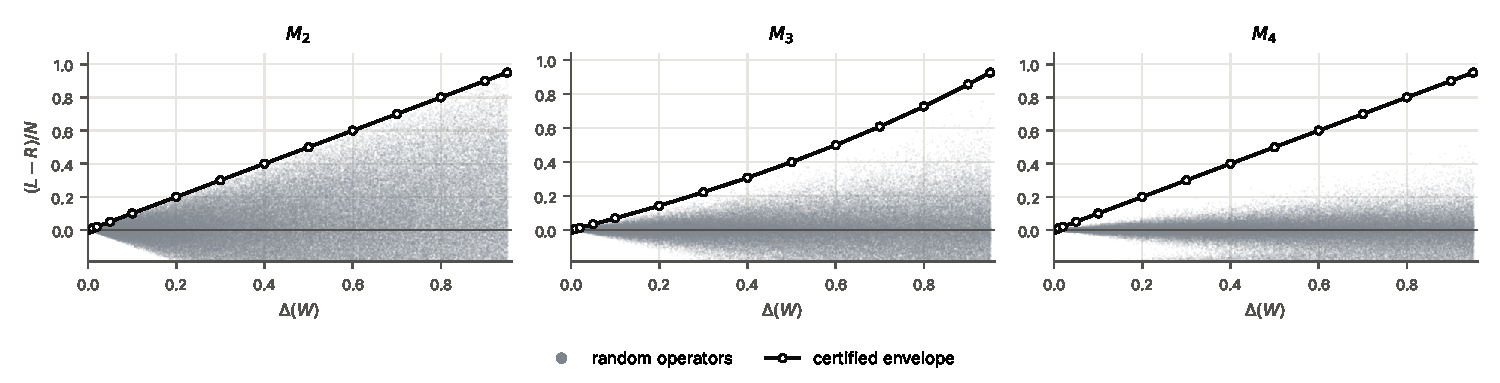
\includegraphics[width=\textwidth]{mc_19_meet.pdf}
\caption[]{Item 19, $\varphi(P+Q)\le\varphi(1+P\wedge Q)$: random samples and the computed envelope (a certified lower bound) against $\Delta(W)$.}
\label{fig:mc-meet}
\end{figure}

\begin{figure}[!htbp]
\centering
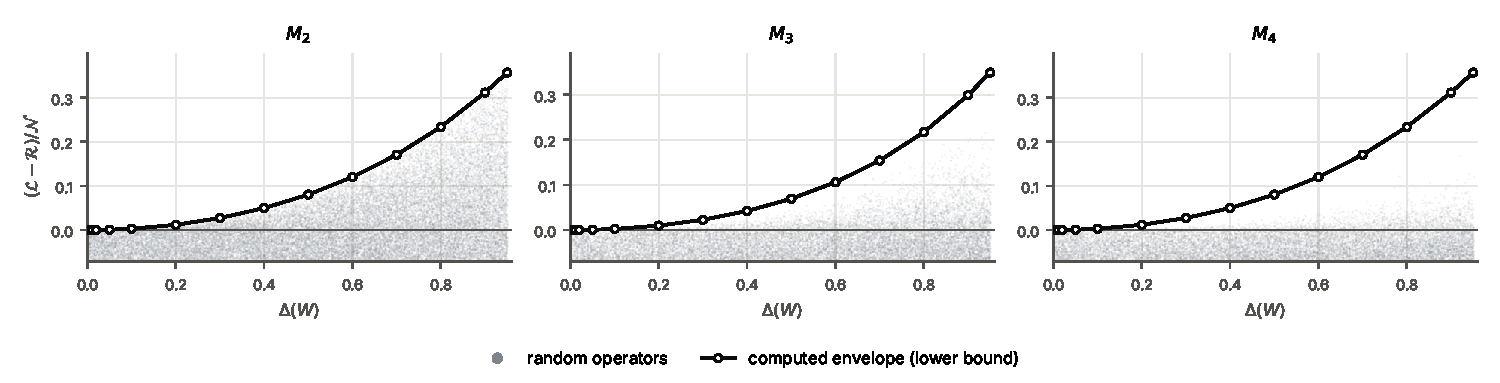
\includegraphics[width=\textwidth]{mc_20_expqpq.pdf}
\caption[]{Item 20, $\varphi(e^{QPQ})\le\varphi(e^P)$: random samples and the computed envelope (a certified lower bound) against $\Delta(W)$.}
\label{fig:mc-expqpq}
\end{figure}

\begin{figure}[!htbp]
\centering
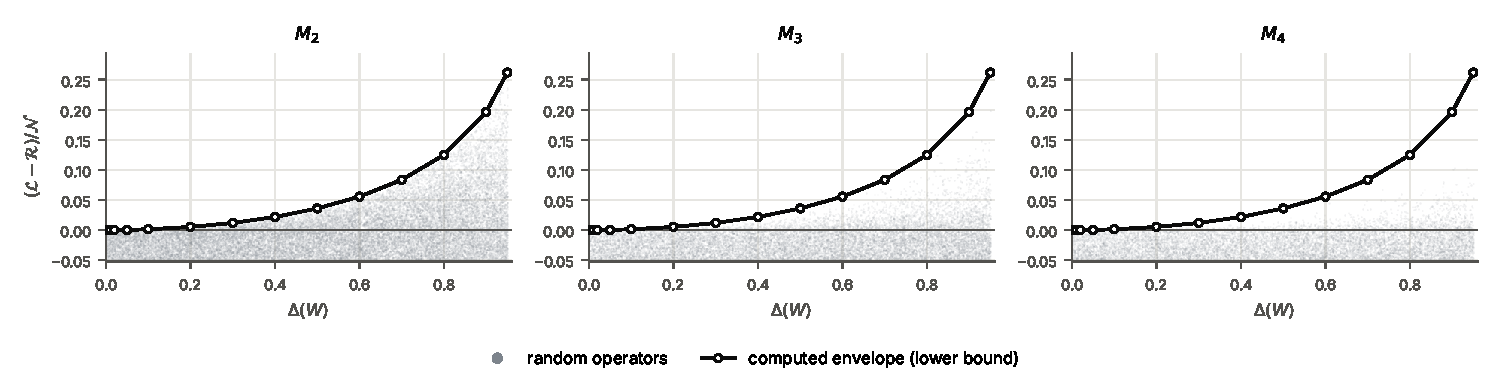
\includegraphics[width=\textwidth]{mc_21_repos.pdf}
\caption[]{Item 21, $\varphi(\mathrm{Re}\,PQ)\ge0$: random samples and the computed envelope (a certified lower bound) against $\Delta(W)$.}
\label{fig:mc-repos}
\end{figure}

\begin{figure}[!htbp]
\centering
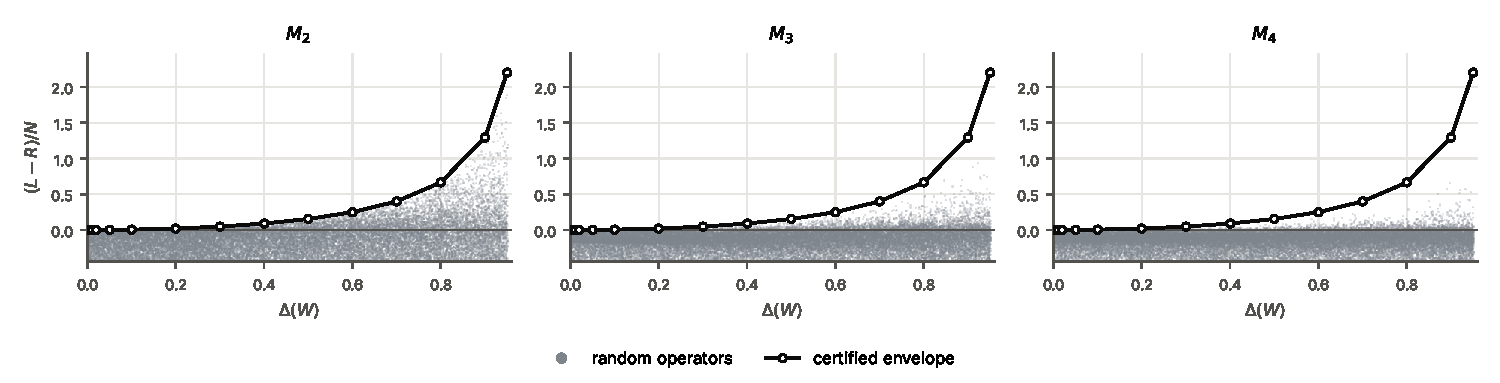
\includegraphics[width=\textwidth]{mc_22_reabs.pdf}
\caption[]{Item 22, $\varphi(\mathrm{Re}\,PQ)\le\varphi(|PQ|)$: random samples and the computed envelope (a certified lower bound) against $\Delta(W)$.}
\label{fig:mc-reabs}
\end{figure}

\begin{figure}[!htbp]
\centering
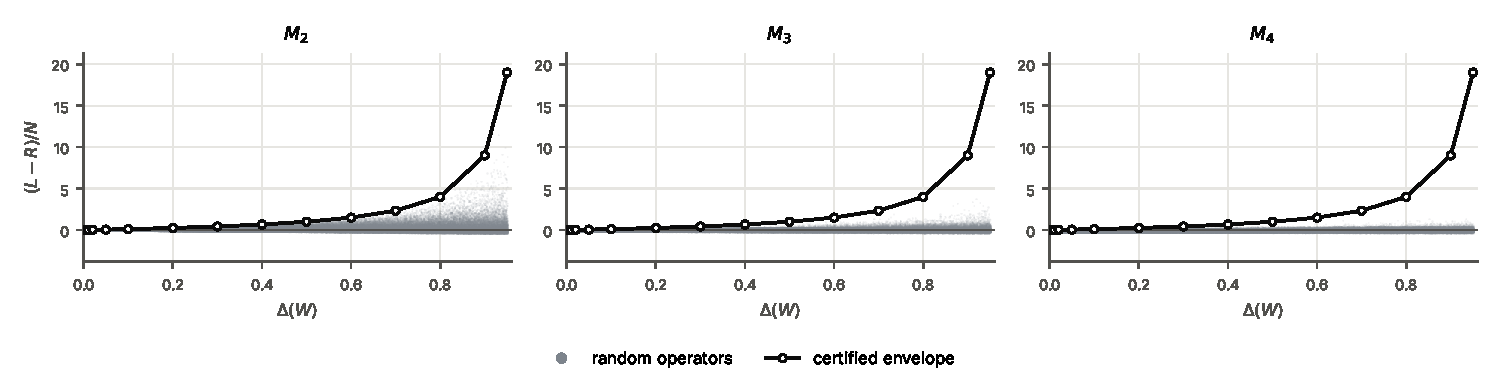
\includegraphics[width=\textwidth]{mc_23_join.pdf}
\caption[]{Item 23, $\varphi(P\vee Q)\le\varphi(P)+\varphi(Q)$: random samples and the computed envelope (a certified lower bound) against $\Delta(W)$.}
\label{fig:mc-join}
\end{figure}

\begin{figure}[!htbp]
\centering
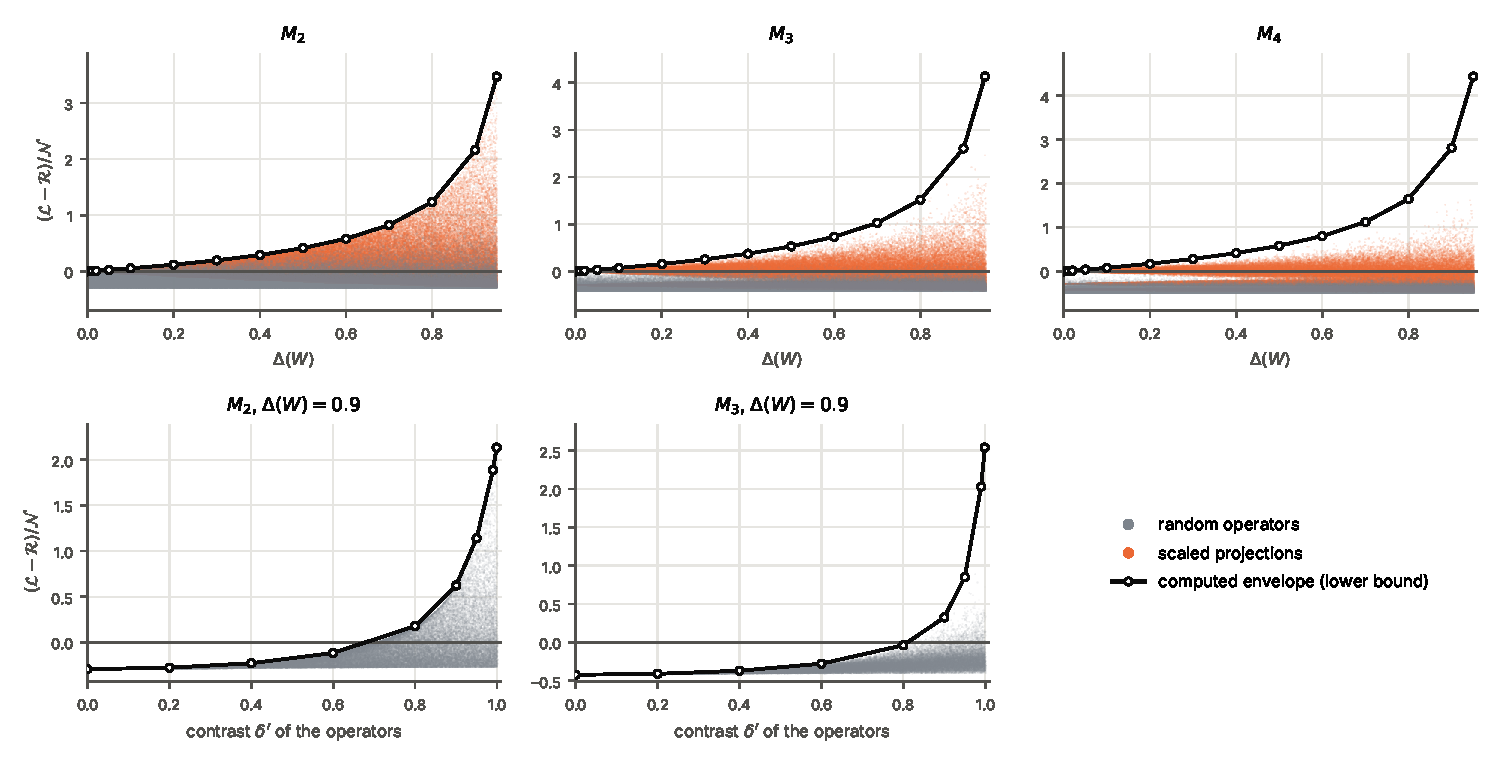
\includegraphics[width=\textwidth]{mc_24_lp.pdf}
\caption[]{Item 24, $\varphi(A^2)^{1/2}\le\varphi(A)$, $\varphi(1)=n$: random samples and the computed envelope (a certified lower bound); top: against $\Delta(W)$, bottom: against the contrast $\delta^\prime$ of the operators at $\Delta(W)=0.9$.}
\label{fig:mc-lp}
\end{figure}

\begin{figure}[!htbp]
\centering
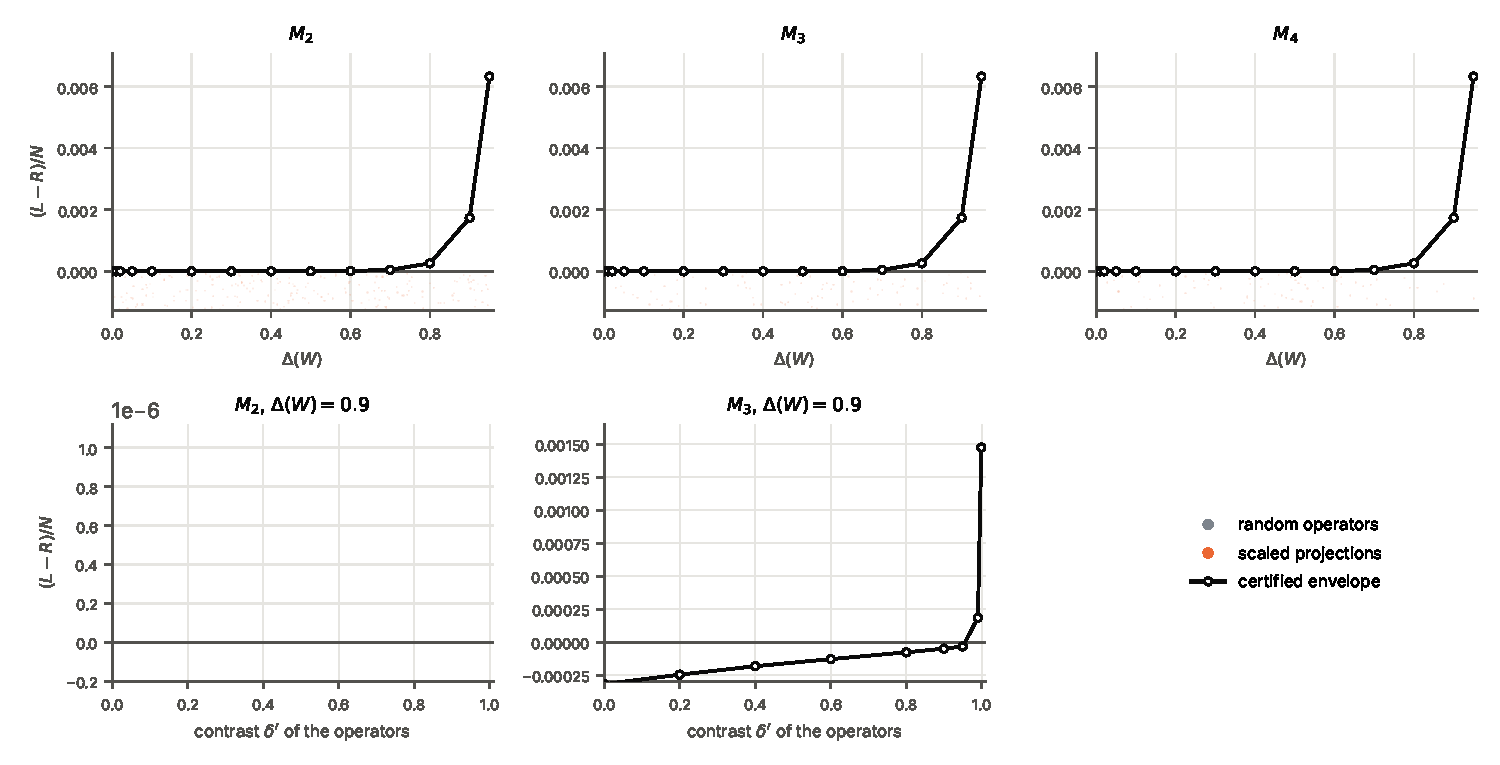
\includegraphics[width=\textwidth]{mc_25_wmon.pdf}
\caption[]{Item 25, $0\le A\le B\Rightarrow\varphi(A^4)\le\varphi(AB^2A)$: random samples and the computed envelope (a certified lower bound); top: against $\Delta(W)$, bottom: against the contrast $\delta^\prime$ of the operators at $\Delta(W)=0.9$.}
\label{fig:mc-wmon}
\end{figure}
